\newpage
\section{Die Samariterin am Brunnen}
\index{Jesus}

\textbf{\textit{C(e,e) | Jesus | Quelle}}
\index{Kommunikation C(e,e)}
\index{Quelle}

\biblerefformat{kurz}
\bibleverse{Joh}(4:5-26)
\begin{BibelSt}
So kam er zu einer Stadt in Samarien, die Sychar hieß und nahe bei dem Grundstück lag, das Jakob seinem Sohn Josef vermacht hatte. Dort befand sich der Jakobsbrunnen. Jesus war müde von der Reise und setzte sich daher an den Brunnen; es war um die sechste Stunde.
Da kam eine Frau aus Samarien, um Wasser zu schöpfen. Jesus sagte zu ihr: Gib mir zu trinken! Seine Jünger waren nämlich in die Stadt gegangen, um etwas zum Essen zu kaufen. Die Samariterin sagte zu ihm: Wie kannst du als Jude mich, eine Samariterin, um etwas zu trinken bitten? Die Juden verkehren nämlich nicht mit den Samaritern. Jesus antwortete ihr: Wenn du wüsstest, worin die Gabe Gottes besteht und wer es ist, der zu dir sagt: Gib mir zu trinken!, dann hättest du ihn gebeten und er hätte dir lebendiges Wasser gegeben. Sie sagte zu ihm: Herr, du hast kein Schöpfgefäß und der Brunnen ist tief; woher hast du also das lebendige Wasser? Bist du etwa größer als unser Vater Jakob, der uns den Brunnen gegeben und selbst daraus getrunken hat, wie seine Söhne und seine Herden? Jesus antwortete ihr: Wer von diesem Wasser trinkt, wird wieder Durst bekommen; wer aber von dem Wasser trinkt, das ich ihm geben werde, wird niemals mehr Durst haben; vielmehr wird das Wasser, das ich ihm gebe, in ihm zu einer Quelle werden, deren Wasser ins ewige Leben fließt. Da sagte die Frau zu ihm: Herr, gib mir dieses Wasser, damit ich keinen Durst mehr habe und nicht mehr hierherkommen muss, um Wasser zu schöpfen!
Er sagte zu ihr: Geh, ruf deinen Mann und komm wieder her! Die Frau antwortete: Ich habe keinen Mann. Jesus sagte zu ihr: Du hast richtig gesagt: Ich habe keinen Mann. Denn fünf Männer hast du gehabt und der, den du jetzt hast, ist nicht dein Mann. Damit hast du die Wahrheit gesagt. Die Frau sagte zu ihm: Herr, ich sehe, dass du ein Prophet bist. Unsere Väter haben auf diesem Berg Gott angebetet; ihr aber sagt, in Jerusalem sei die Stätte, wo man anbeten muss. Jesus sprach zu ihr: Glaube mir, Frau, die Stunde kommt, zu der ihr weder auf diesem Berg noch in Jerusalem den Vater anbeten werdet. Ihr betet an, was ihr nicht kennt, wir beten an, was wir kennen; denn das Heil kommt von den Juden. Aber die Stunde kommt und sie ist schon da, zu der die wahren Beter den Vater anbeten werden im Geist und in der Wahrheit; denn so will der Vater angebetet werden. Gott ist Geist und alle, die ihn anbeten, müssen im Geist und in der Wahrheit anbeten. Die Frau sagte zu ihm: Ich weiß, dass der Messias kommt, der Christus heißt. Wenn er kommt, wird er uns alles verkünden. Da sagte Jesus zu ihr: Ich bin es, der mit dir spricht.
\end{BibelSt}

\subsection{Impuls}
\begin{figure}
    \centering
    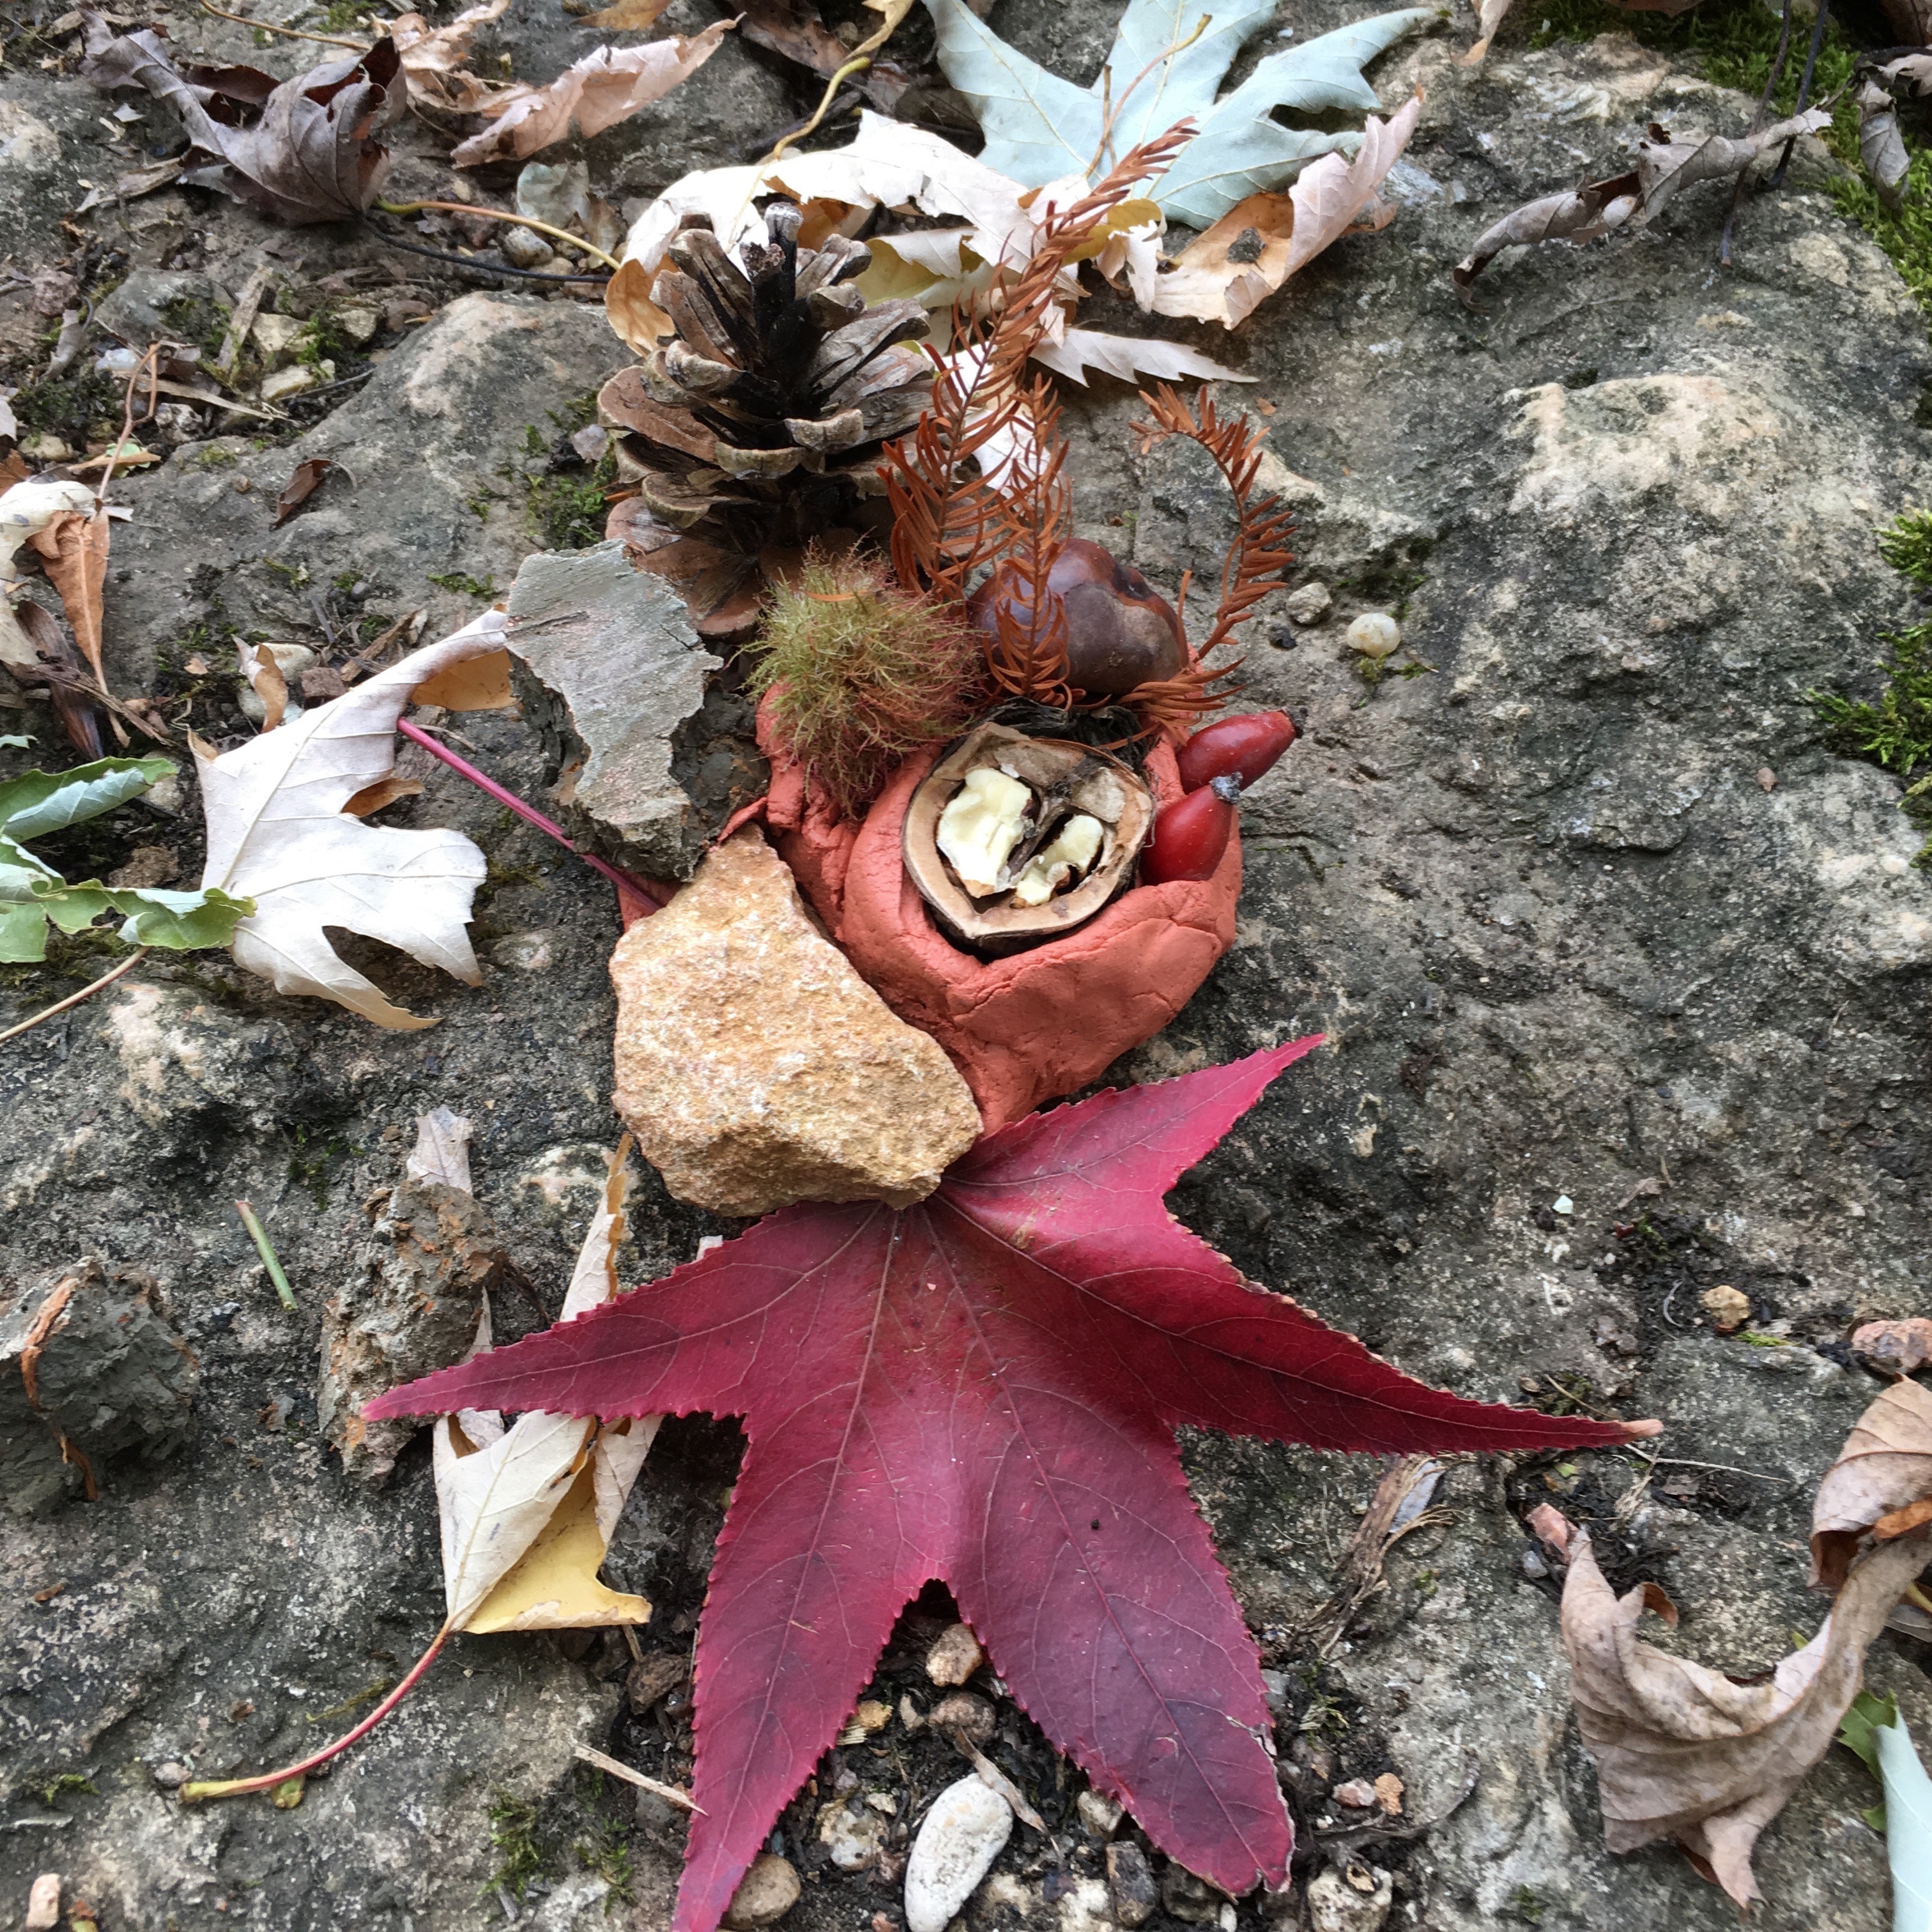
\includegraphics[scale=0.09]
{Pictures/2018-10-Gottesbild-Taize.jpg}
    \caption{Gottesbild, 25. Oktober 2018, Taizé}
    \label{fig:Bildmeditation}
\end{figure}
\begin{impuls}
\begin{description}
 \item[Gottesbilder: bei der Quelle]
 \begin{gedicht}
 \begin{verse}
 \\!
 Taizé — Pilgerweg des Vertrauens in einen Gott,  der für mich Geist — Energie, Wind — ist. Das Unfassbare ist mir am nächsten.\\!
 
Aus Erde geschaffen. Was lässt sich aus diesem Ton formen?\\!

Aufmerksam werden, für das, was mir am Wegrand geschenkt wird: Stein, Kastanie. 
Erinnerung an frühere Stationen auf dem Pilgerweg hier in Taizé. Den Ton formen um zu fassen, was mir am Wegrand geschenkt wird.\\
Nuss — ihr Kern enthält alles, um ein grosser, starker Baum zu werden. Tannzapfen, rote Blätter… Erinnerungen. Vergängliche Schönheit des Herbstes, selbst im Unkraut.\\!

Ich wollte zur Quelle kommen, doch der Teich ist ausgetrocknet. In der Ferne schwingt der Psalm mit: «Wie der Hirsch lechzt nach frischem Wasser»… Ausgetrockneter Teich, Lehmboden. Aus der Erde geschaffen … kein Meissen-Porzellan. Der Versuch, in dem instabilen Gefäss zu fassen, was mir geschenkt wird. \\!

Zerbrechlich. Vergänglich.\\!

Echo einer Bibelstelle: Was weiss der Ton über seinen Schöpfer? 
Sich kein Bild von Gott machen. Und nun forme ich nicht Gott, sondern meine zu ahnen, wie Gott mich formen möchte.\\!
 \end{verse}
 \end{gedicht}
 \item[Auf dem Weg und beim Gotteswortgärtchen] 
 \begin{gedicht}
 \begin{verse}
 \\!
 Vergänglich die Geschenke, zerbrechlich der Ton. Gehärtet im Wind und Feuer des Geistes, und doch zerbrechlich. Der Versuch, zusammenzuhalten. Wissen um die Vergänglichkeit, und doch das Zerbrechen verhindern — hinauszögern.\\!
 
Getragen in der Hand des Schöpfers. Getragen sein. Tragen. Weitergehen auf dem Pilgerweg des Vertrauens zu meinem Gotteswortgärtchen.\\!

Ikone der Begegnung mit der Samariterin am Brunnen. Das Echo des lebendigen Wassers nach der ausgetrockneten Quelle. Tränen. Erinnerungen.\\!

Mein Gottesbild auf dem Pilgerweg des Vertrauens, gewickelt in Zeitungspapier, in eine Kartonschachtel gelegt. Eine Krippe? Wird hier ein neues Gottesbild geboren?
\end{verse}
 \end{gedicht}
\end{description}
\end{impuls}

\subsection{die samariterin am brunnen}
\cite{KHH} vom 17.3
\begin{gedicht}
\begin{verse}
sie sagen, ich sei eine hure.\\
ein leichtes mädchen\\
ich mit meinen stöckelschuhen\\
den klingenden armbändern\\
dem roten kleid und dem weigenden gang\\
sie gehn mir aus dem weg\\
wenigstens tagsüber\\!

darum laufe ich\\
in der hitze zum brunnen\\
ich ertrage die blicke\\
der frauen nicht\\!

jetzt bist du da\\
fremder mann\\
du batest um einen schluck wasser\\
du, der fremde\\!

nicht die hure sahst du in mir\\
nicht die frau\\
nicht die fremde und andersgläubige\\
su sahst in mir den menschen\\
der hinter der schminke weint\\
und gabst mir aus deiner quelle\\
wasser des heils und der vergebung\\
auf dass ich lebe\\
und alle herbeirufe\\
zu deinem brunnen
\end{verse}
\end{gedicht}

\subsection{Lied: De noche (12)}
De noche iremos, de noche que para encontrar la fuente, solo la sed nos alumbra, solo la sed nos alumbra.
